\hypertarget{bootstrap-sampling}{%
\chapter{Bootstrap Sampling}\label{bootstrap-sampling}}

In the previous chapter we used resampling to compute standard errors
and confidence intervals, which quantify the variability in an estimate
due to random sampling. As one of the examples, we used data from the
General Social Survey (GSS) to explore changes in support for gun
control over time and to compute confidence intervals for the estimated
proportions.

In this chapter, we'll use GSS data to estimate average income and the
10th percentile of income. We'll see that the resampling method we used
in the previous chapter works for the average income but not for the
10th percentile.

To solve this problem, we'll use another kind of resampling, called
bootstrapping or bootstrap sampling (see
\url{https://en.wikipedia.org/wiki/Bootstrapping_(statistics)}). Then
we'll use bootstrapping to compute sampling distributions and confidence
intervals for other statistics, including the coefficient of correlation
and the parameters of linear regression. Finally, I'll point out a
problem with bootstrap resampling when there are not enough different
values in a dataset, and a way to solve it with KDE resampling.

\hypertarget{estimating-average-income}{%
\section{Estimating Average Income}\label{estimating-average-income}}

As a first example, we'll use data from the General Social Survey to
estimate average family income. The following cell loads the data, which
I have stored in an HDF file.

\begin{lstlisting}[]
import pandas as pd

gss = pd.read_hdf('gss_eda.hdf', 'gss')
gss.head()
\end{lstlisting}

\begin{tabular}{lrrrrrrrr}
\midrule
{} &  YEAR &  ID\_ &   AGE &  EDUC &  SEX &  GUNLAW &  GRASS &  REALINC \\
\midrule
0 &  1972 &    1 &  23.0 &  16.0 &    2 &     1.0 &    NaN &  18951.0 \\
1 &  1972 &    2 &  70.0 &  10.0 &    1 &     1.0 &    NaN &  24366.0 \\
2 &  1972 &    3 &  48.0 &  12.0 &    2 &     1.0 &    NaN &  24366.0 \\
3 &  1972 &    4 &  27.0 &  17.0 &    2 &     1.0 &    NaN &  30458.0 \\
4 &  1972 &    5 &  61.0 &  12.0 &    2 &     1.0 &    NaN &  50763.0 \\
\midrule
\end{tabular}

The column \passthrough{\lstinline!REALINC!} records family income,
converted to 1986 dollars. We can use \passthrough{\lstinline!notna!}
and \passthrough{\lstinline!sum!} to count the number of valid
responses.

\begin{lstlisting}[]
n_realinc = gss['REALINC'].notna().sum()
n_realinc
(@\dashfill@)
@@@58293@@@
\end{lstlisting}

And we can compute the mean and standard deviation of the valid
responses.

\begin{lstlisting}[]
mean_realinc = gss['REALINC'].mean()
std_income = gss['REALINC'].std()
print(mean_realinc, std_income)
(@\dashfill@)
@@@31742.563372816312 29526.067896235618@@@
\end{lstlisting}

The average family income in this dataset is \$31,742. But notice that
the standard deviation is almost equal to the mean. That's because the
distribution of income is long-tailed; many families have incomes below
the mean, and there are a few families with incomes much higher than the
mean. Nevertheless, we can use this function from the previous chapter
to simulate the sampling process.

\begin{lstlisting}[]
import numpy as np

def simulate_sample_mean(n, mu, sigma):
    sample = np.random.normal(mu, sigma, size=n)
    return sample.mean()
\end{lstlisting}

\passthrough{\lstinline!simulate\_sample\_mean!} takes as parameters the
sample size, \passthrough{\lstinline!n!}, and the presumed mean and
standard deviation of income. It generates a sample from a normal
distribution with the given mean and standard deviation, and returns the
mean of the sample. If we call it once, we get a random value from the
sampling distribution of the mean.

\begin{lstlisting}[]
simulate_sample_mean(n_realinc, mean_realinc, std_income)
(@\dashfill@)
@@@31791.715011882538@@@
\end{lstlisting}

If we call it many times, we get a random sample from the sampling
distribution.

\begin{lstlisting}[]
t1 = [simulate_sample_mean(n_realinc, mean_realinc, std_income)
     for i in range(1000)]
\end{lstlisting}

I'll use the following function to summarize the sampling distribution.

\begin{lstlisting}[]
def summarize(t, digits=2):
    table = pd.DataFrame(columns=['Estimate', 'SE', 'CI90'])
    est = np.mean(t).round(digits)
    SE = np.std(t).round(digits)
    CI90 = np.percentile(t, [5, 95]).round(digits)
    table.loc[''] = est, SE, CI90
    return table
\end{lstlisting}

\begin{lstlisting}[]
summary1 = summarize(t1, digits=1)
summary1
\end{lstlisting}

\begin{tabular}{lrrl}
\midrule
{} &  Estimate &     SE &                CI90 \\
\midrule
{} &   31733.4 &  126.5 &  [31526.3, 31937.7] \\
\midrule
\end{tabular}

The result is a table that shows the mean of the sampling distribution,
the standard error, and a 90\% confidence interval. The mean of the
sampling distribution is consistent with the mean of the data, which is
\$31,743.

\hypertarget{estimating-percentiles}{%
\section{Estimating Percentiles}\label{estimating-percentiles}}

The method in the previous section uses a normal distribution to
simulate the sampling process. In the previous chapter, when we
estimated average height, this worked well because human heights are
well modeled by a normal distribution. But income is not. We can see
that by computing the CDF of a normal distribution with the same mean
and standard as the income data.

\begin{lstlisting}[]
from scipy.stats import norm

xs = np.linspace(-40000, 150000)
ys = norm(mean_realinc, std_income).cdf(xs)
\end{lstlisting}

And comparing it to the CDF of the data.

\begin{lstlisting}[]
from empiricaldist import Cdf

cdf_realinc = Cdf.from_seq(gss['REALINC'])
\end{lstlisting}

\begin{lstlisting}[]
import matplotlib.pyplot as plt

plt.plot(xs, ys, color='0.7', label='normal model')
cdf_realinc.plot(label='GSS data')

plt.xlabel('Family income (1986 $)')
plt.ylabel('CDF')
plt.title('Distribution of income')
plt.legend();
\end{lstlisting}

\begin{center}
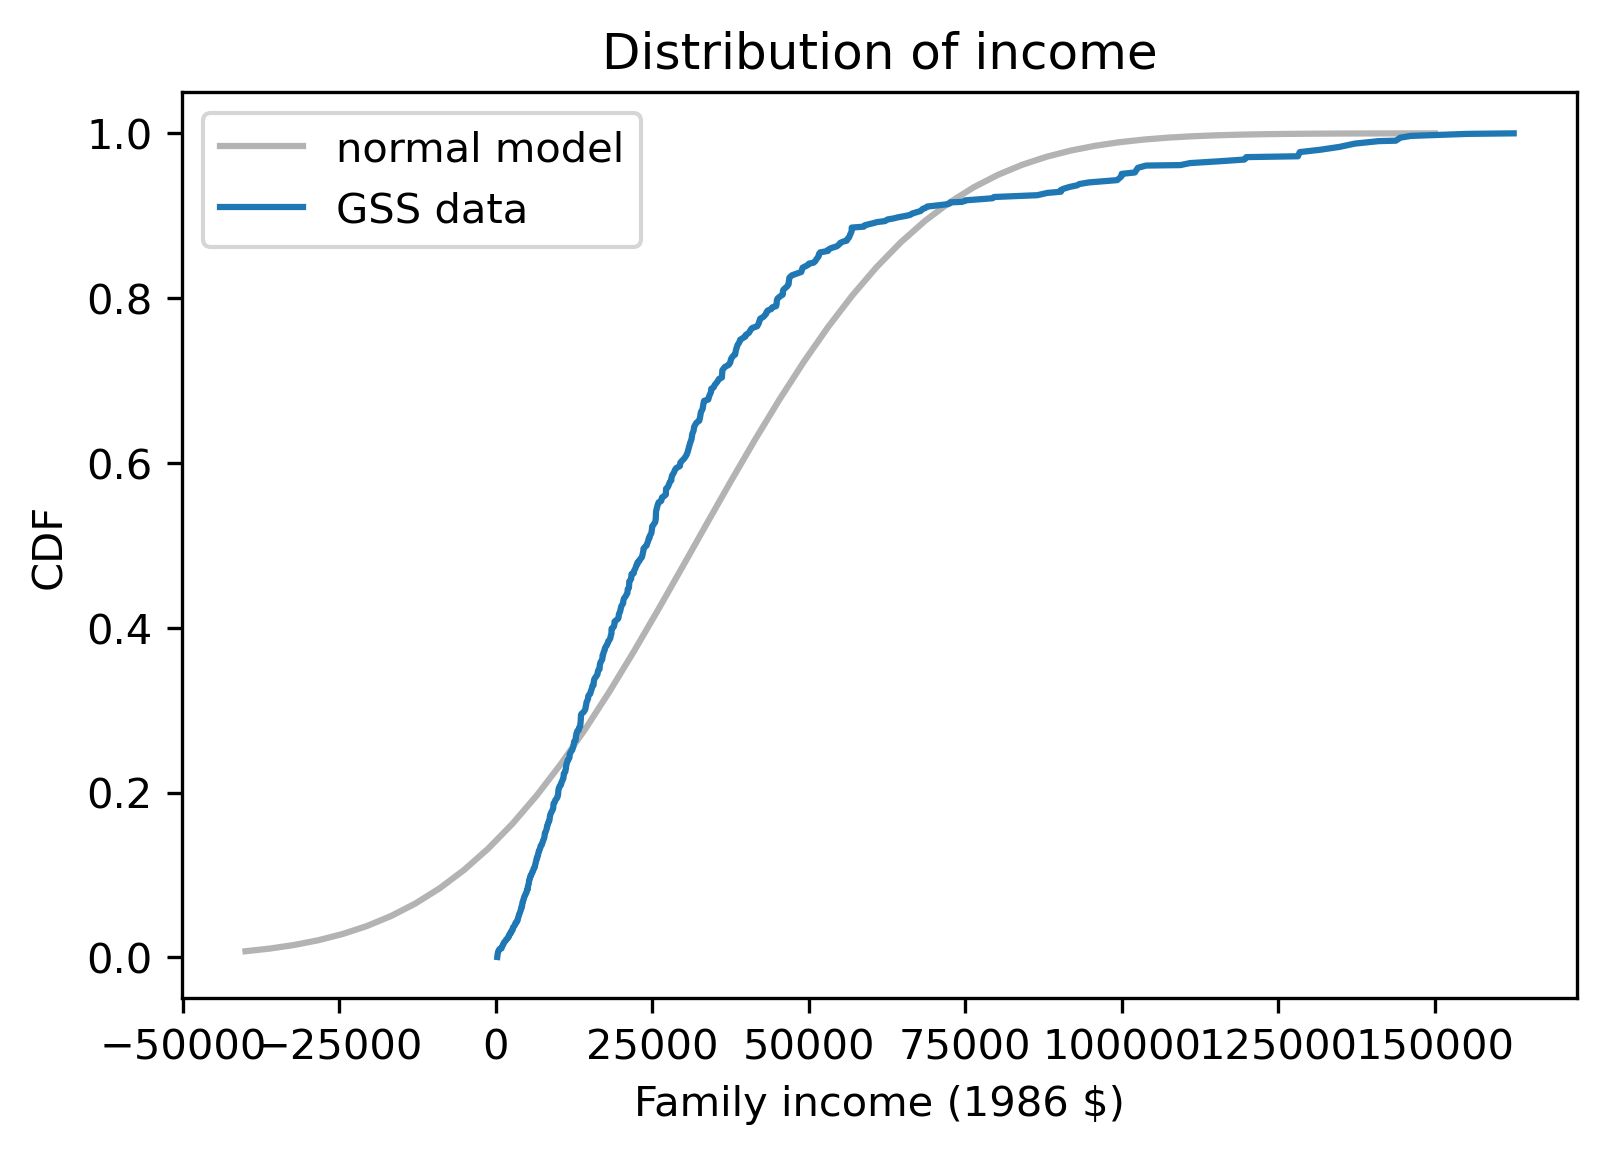
\includegraphics[width=4in]{12_bootstrap_files/12_bootstrap_29_0.png}
\end{center}

The normal distribution is not a good model for the data. As we saw in
the previous section, it is good enough to compute the sampling
distribution of the mean. But for other statistics, like percentiles, it
is not good enough. To demonstrate, here's a function that generates a
sample from a normal distribution and returns the 10th percentile.

\begin{lstlisting}[]
def simulate_sample_percentile(n, mu, sigma):
    sample = np.random.normal(mu, sigma, size=n)
    return np.percentile(sample, 10)
\end{lstlisting}

We can use it to generate a sample from the sampling distribution of the
10th percentile.

\begin{lstlisting}[]
t2 = [simulate_sample_percentile(n_realinc, mean_realinc, std_income)
      for i in range(1000)]
\end{lstlisting}

Here's a summary of the results.

\begin{lstlisting}[]
summary2 = summarize(t2)
summary2
\end{lstlisting}

\begin{tabular}{lrrl}
\midrule
{} &  Estimate &      SE &                 CI90 \\
\midrule
{} &  -6099.36 &  212.86 &  [-6445.8, -5742.18] \\
\midrule
\end{tabular}

The mean of the sampling distribution is negative, which is not
consistent with the actual 10th percentile of the data, which is \$5631.

In this example, resampling based on a normal model doesn't produce
sensible results. Fortunately there is a simple alternative that is more
robust: bootstrapping.

\hypertarget{bootstrapping}{%
\section{Bootstrapping}\label{bootstrapping}}

Bootstrapping is a kind of resampling, based on the framework we saw in
the previous chapter:

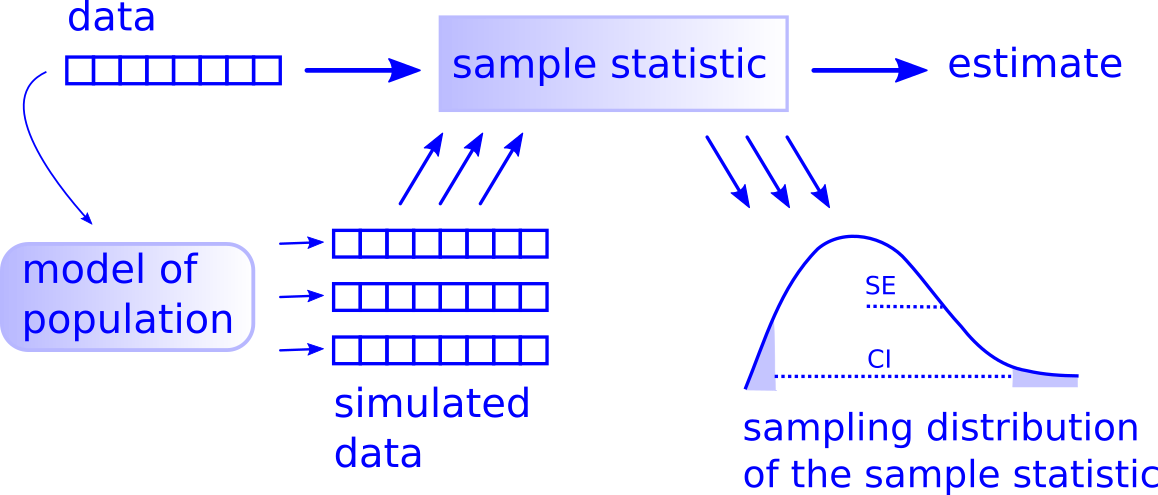
\includegraphics{figs/resampling.png}

The idea is that we treat the sample as if it were the entire
population, and simulate the sampling process by choosing random rows
with replacement. \passthrough{\lstinline!DataFrame!} provides a method
called \passthrough{\lstinline!sample!} we can use to select a random
sample of the rows.

\begin{lstlisting}[]
bootstrapped = gss.sample(n=n_realinc, replace=True)
bootstrapped.shape
(@\dashfill@)
@@@(58293, 8)@@@
\end{lstlisting}

The argument \passthrough{\lstinline!n=n\_realinc!} means that the
bootstrapped sample has the same size as the original.

\passthrough{\lstinline!replace=True!} means that sampling is done with
replacement; that is, the same row can be chosen more than once. To see
how many times each row appears in the bootstrapped sample, we can use
\passthrough{\lstinline!value\_counts!} and the
\passthrough{\lstinline!\_ID!} column, which contains a unique
identifier for each respondent.

\begin{lstlisting}[]
repeats = bootstrapped['ID_'].value_counts()
repeats.head()
\end{lstlisting}

\begin{tabular}{lr}
\midrule
{} &  ID\_ \\
\midrule
1158 &   50 \\
1427 &   44 \\
1367 &   44 \\
1029 &   44 \\
1119 &   44 \\
\midrule
\end{tabular}

Since some rows appear many times, other rows don't appear at all. To
see how many, we can use \passthrough{\lstinline!set!} subtraction to
count the values of \passthrough{\lstinline!ID\_!} that appear in the
original dataset but not the bootstrapped sample.

\begin{lstlisting}[]
unused = set(gss['ID_']) - set(bootstrapped['ID_'])
len(unused)
(@\dashfill@)
@@@560@@@
\end{lstlisting}

Now we can use bootstrapping to generate a sampling distribution. For
example, the following function takes a
\passthrough{\lstinline!DataFrame!}, generates a bootstrapped sample,
and returns the average income.

\begin{lstlisting}[]
def bootstrap_mean(df, varname):
    bootstrapped = df.sample(n=len(df), replace=True)
    return bootstrapped[varname].mean()
\end{lstlisting}

If we run it many times, we get a sample from the sampling distribution
of the mean.

\begin{lstlisting}[]
t3 = [bootstrap_mean(gss, 'REALINC')
      for i in range(1001)]
\end{lstlisting}

Here's a summary of the results, compared to the results based on the
normal model.

\begin{lstlisting}[]
summary3 = summarize(t3)
table = pd.concat([summary1, summary3])
table.index=['normal model', 'bootstrapping']
table
\end{lstlisting}

\begin{tabular}{lrrl}
\midrule
{} &  Estimate &      SE &                 CI90 \\
\midrule
normal model  &  31733.40 &  126.50 &   [31526.3, 31937.7] \\
bootstrapping &  31742.15 &  121.81 &  [31543.9, 31946.88] \\
\midrule
\end{tabular}

The results from bootstrap sampling are consistent with the results
based on the normal model. Now let's see what happens when we estimate
the 10th percentile.

The following function generates a bootstrapped sample and returns the
10th percentile. Instead of \passthrough{\lstinline!percentile!} from
Numpy, it uses \passthrough{\lstinline!quantile!} from Pandas, which
drops \passthrough{\lstinline!NaN!} values. The parameter of
\passthrough{\lstinline!quantile!} is a probability between 0 and 1,
rather than a percentage between 0 and 100.

\begin{lstlisting}[]
def bootstrap_percentile(df):
    bootstrapped = df.sample(n=len(df), replace=True)
    return bootstrapped['REALINC'].quantile(0.1)
\end{lstlisting}

We can use it to generate a sample from the sampling distribution of the
10th percentile.

\begin{lstlisting}[]
t4 = [bootstrap_percentile(gss)
      for i in range(1001)]
\end{lstlisting}

Here are the results along with the results based on the normal model.

\begin{lstlisting}[]
summary4 = summarize(t4)
table = pd.concat([summary2, summary4])
table.index=['normal model', 'bootstrapping']
table
\end{lstlisting}

\begin{tabular}{lrrl}
\midrule
{} &  Estimate &      SE &                 CI90 \\
\midrule
normal model  &  -6099.36 &  212.86 &  [-6445.8, -5742.18] \\
bootstrapping &   5646.45 &   85.93 &     [5512.5, 5806.0] \\
\midrule
\end{tabular}

The mean of the sampling distribution is consistent with the 10th
percentile of the data, which is \$5631. So the results from
bootstrapping are more sensible than the results based on the normal
model.

In general, bootstrapping is robust; that is, it works well with many
different distributions and many different statistics. However, at the
end of the chapter, we'll see one example where it fails.

\hypertarget{bigger-data}{%
\section{Bigger Data}\label{bigger-data}}

As sample size increases, errors due to random sampling get smaller. To
demonstrate this effect, I'll use data from the Behavioral Risk Factor
Surveillance System (BRFSS).

In previous chapters, we used BRFSS data to explore the relationship
between height and weight, and the relationship between income and
vegetable consumption. In this section, we'll use it to estimate the
average height for men in the United States.

First, let's read the 2019 data, which I have stored in an HDF file.

\begin{lstlisting}[]
import pandas as pd

brfss = pd.read_hdf('brfss.hdf', 'brfss')
brfss.shape
(@\dashfill@)
@@@(418268, 9)@@@
\end{lstlisting}

This dataset contains 418 268 rows, one for each respondent, and 11
columns, one for each variable I selected. Here are the first few rows.

\begin{lstlisting}[]
brfss.head()
\end{lstlisting}

\begin{tabular}{lrrrrrrrrr}
\midrule
{} &       SEQNO &   HTM4 &  WTKG3 &  \_SEX &  \_AGEG5YR &  \_VEGESU1 &  \_INCOMG &      \_LLCPWT &   AGE \\
\midrule
0 &  2019000001 &  157.0 &  69.85 &     2 &      13.0 &     114.0 &        2 &   135.304080 &  82.0 \\
1 &  2019000002 &  163.0 &  48.99 &     2 &      11.0 &     121.0 &        3 &  1454.882220 &  72.0 \\
2 &  2019000003 &  165.0 &  86.18 &     2 &      10.0 &     164.0 &        5 &   215.576852 &  67.0 \\
3 &  2019000004 &  165.0 &  55.34 &     2 &      13.0 &       NaN &        4 &   261.282838 &  82.0 \\
4 &  2019000005 &  152.0 &  49.90 &     2 &      13.0 &     178.0 &        9 &   535.270103 &  82.0 \\
\midrule
\end{tabular}

Here's a Boolean \passthrough{\lstinline!Series!} that's
\passthrough{\lstinline!True!} for male respondents.

\begin{lstlisting}[]
male = (brfss['_SEX'] == 1)
male.sum()
(@\dashfill@)
@@@189835@@@
\end{lstlisting}

The column \passthrough{\lstinline!HTM4!} contains their heights in
centimeters.

\begin{lstlisting}[]
height = brfss['HTM4']
\end{lstlisting}

We can use \passthrough{\lstinline!notna!} and
\passthrough{\lstinline!sum!} to count the number of rows with valid
height data.

\begin{lstlisting}[]
n_height = height[male].notna().sum()
n_height
(@\dashfill@)
@@@182269@@@
\end{lstlisting}

There are 182 269 male respondents with known heights. Here is the mean
and standard deviation of these values.

\begin{lstlisting}[]
mean_height = height[male].mean()
std_height = height[male].std()
mean_height, std_height
(@\dashfill@)
@@@(178.0768644146838, 7.966455313471575)@@@
\end{lstlisting}

The average height for men in the U.S. is about 178.1 cm; the standard
deviation is about 8 cm. We can use bootstrapping to generate values
from the sampling distribution of the mean. To reduce computation time,
I reduced the number of iterations to 201.

\begin{lstlisting}[]
t5 = [bootstrap_mean(brfss[male], 'HTM4')
      for i in range(201)]

summarize(t5, digits=3)
\end{lstlisting}

\begin{tabular}{lrrl}
\midrule
{} &  Estimate &    SE &                CI90 \\
\midrule
{} &   178.078 &  0.02 &  [178.038, 178.109] \\
\midrule
\end{tabular}

Because the sample size is so large, the standard error is small and the
confidence interval is narrow. This result suggests that our estimate is
very precise, which is true in the sense that the error due to random
sampling is small.

But there are other sources of error. For example, the heights and
weights in this dataset are based on self-reports, so they are
vulnerable to \textbf{social desirability bias} (see
\url{https://en.wikipedia.org/wiki/Social-desirability_bias}). It's also
possible that there are errors in recording the data. In a previous year
of the BRFSS, there are a suspicious number of heights recorded as 60 or
61 centimeters. I suspect that many of them are six feet, or six feet
and one inch, and something went wrong in the preparation of the data.

And that brings us to the first point of this example:

\begin{quote}
With large sample sizes, error due to random sampling is small, but with
real-world data, that usually means that there are other sources of
error that are bigger. So we can't be sure that the estimate is
accurate.
\end{quote}

In fact, there is another source of error in this example that we have
not taken into account: oversampling.

\hypertarget{weighted-bootstrapping}{%
\section{Weighted Bootstrapping}\label{weighted-bootstrapping}}

By design, the BRFSS oversamples some groups; that is, people in some
groups are more likely than others to appear in the sample. If people in
these groups are taller than others on average, or shorter, our
estimated mean would not be accurate.

We encountered this issue in Chapter 7, where we used data from the
National Survey of Family Growth (NSFG) to compute the average birth
weight for babies in the United States. In that example, we corrected
for oversampling by computing a weighted mean.

In this example, we will use a different method, \textbf{weighted
bootstrapping}, to estimate the mean and compute a confidence interval.

The BRFSS dataset includes a column, \passthrough{\lstinline!\_LLCPWT!},
that contains sampling weights. The sampling weight for each respondent
is the number of people in the population they represent. People in
oversampled groups have lower sampling weights; people in undersampled
groups have higher sampling weights. Here's what the range of values
looks like.

\begin{lstlisting}[]
brfss['_LLCPWT'].describe()
\end{lstlisting}

\begin{tabular}{lr}
\midrule
{} &        \_LLCPWT \\
\midrule
count &  418268.000000 \\
mean  &     603.513276 \\
std   &    1082.430311 \\
min   &       1.016173 \\
25\%   &     111.160528 \\
50\%   &     272.869258 \\
75\%   &     654.211787 \\
max   &   42066.730900 \\
\midrule
\end{tabular}

The lowest sampling weight is about 1; the largest is 42 066. So that's
a very wide range!

We can take these weights into account by passing them as an argument to
\passthrough{\lstinline!sample!}. That way, the probability that any row
is selected is proportional to its sampling weight.

\begin{lstlisting}[]
n = len(brfss)
bootstrapped = brfss.sample(n=n, replace=True, weights='_LLCPWT')
\end{lstlisting}

As we saw with unweighted bootstrapping, the same row can appear more
than once. To see how many times, we can use
\passthrough{\lstinline!value\_counts!} and the
\passthrough{\lstinline!SEQNO!} column, which contains a unique
identifier for each respondent.

\begin{lstlisting}[]
repeats = bootstrapped['SEQNO'].value_counts()
repeats.head()
\end{lstlisting}

\begin{tabular}{lr}
\midrule
{} &  SEQNO \\
\midrule
2019000108 &    134 \\
2019000851 &    130 \\
2019006167 &    123 \\
2019000096 &    122 \\
2019000047 &    119 \\
\midrule
\end{tabular}

Some rows appear more than 100 times. Most likely, these are the rows
with the highest sampling rates, which correspond to people from
undersampled groups.

To see how many rows don't appear at all, we can use
\passthrough{\lstinline!set!} subtraction to count the values of
\passthrough{\lstinline!SEQNO!} that appear in the original dataset but
not the sample.

\begin{lstlisting}[]
unused = set(brfss['SEQNO']) - set(bootstrapped['SEQNO'])
len(unused)
(@\dashfill@)
@@@817@@@
\end{lstlisting}

There are several hundred rows that don't appear in this sample, but
they are not dropped altogether; when we repeat this process, they will
appear in other samples.

We can use weighted bootstrapping to generate values from the sampling
distribution of the mean. The following function uses
\passthrough{\lstinline!sample!} and the
\passthrough{\lstinline!\_LLCPWT!} column to generate a bootstrapped
sample, then returns the average height.

\begin{lstlisting}[]
def weighted_bootstrap_mean(df):
    n = len(df)
    sample = df.sample(n=n, replace=True, weights='_LLCPWT')
    return sample['HTM4'].mean()
\end{lstlisting}

I'll test this function with a \passthrough{\lstinline!DataFrame!} that
contains only male respondents. If we run it once, we get a random value
from the sampling distribution of the weighted mean.

\begin{lstlisting}[]
male_df = brfss[male]
weighted_bootstrap_mean(male_df)
(@\dashfill@)
@@@177.6096682823134@@@
\end{lstlisting}

If we run it many times, we get a random sample from the sampling
distribution.

\begin{lstlisting}[]
t6 = [weighted_bootstrap_mean(male_df) 
      for i in range(201)]

summarize(t6, digits=3)
\end{lstlisting}

\begin{tabular}{lrrl}
\midrule
{} &  Estimate &     SE &                CI90 \\
\midrule
{} &   177.641 &  0.021 &  [177.605, 177.678] \\
\midrule
\end{tabular}

The mean of the sampling distribution estimates the average height for
men in the U.S., corrected for oversampling. If we compare it to the
unweighted mean we computed, it is a little lower.

\begin{lstlisting}[]
print(np.mean(t6), mean_height)
(@\dashfill@)
@@@177.6410065054404 178.0768644146838@@@
\end{lstlisting}

So it seems like people in the oversampled groups are taller than
others, on average, by enough to bring the unweighted mean up by about
half a centimeter.

The difference between the weighted and unweighted means is bigger than
the width of the confidence interval. So in this example the error if we
fail to correct for oversampling is bigger than variability due to
random sampling.

\hypertarget{correlation-and-regression}{%
\section{Correlation and Regression}\label{correlation-and-regression}}

Bootstrap resampling can be used to estimate other statistics and their
sampling distributions. For example, in Chapter 9 we computed the
correlation between height and weight, which is about 0.48.

\begin{lstlisting}[]
var1, var2 = 'HTM4', 'WTKG3'
corr = brfss[var1].corr(brfss[var2])
corr
(@\dashfill@)
@@@0.47715146283881427@@@
\end{lstlisting}

That correlation does not take into account oversampling. We can correct
it with this function, which generates a weighted bootstrapped sample
and uses it to compute the correlation of the columns with names
\passthrough{\lstinline!var1!} and \passthrough{\lstinline!var2!}.

\begin{lstlisting}[]
def weighted_bootstrap_corr(df, var1, var2):
    n = len(df)
    sample = df.sample(n=n, replace=True, weights='_LLCPWT')
    corr = sample[var1].corr(sample[var2])
    return corr
\end{lstlisting}

\textbf{Exercise:} Use this function to draw 101 values from the
sampling distribution of the correlation between height and weight. What
is the mean of these values? Is it substantially different from the
correlation we computed without correcting for oversampling? Compute the
standard error and 90\% confidence interval for the estimated
correlation.

\textbf{Exercise:} In Chapter 9 we also computed the slope of the
regression line for weight as a function of height. Here's the result
with with 2019 data.

\begin{lstlisting}[]
from scipy.stats import linregress

subset = brfss.dropna(subset=['WTKG3', 'HTM4'])
res = linregress(subset['HTM4'], subset['WTKG3'])
res.slope
(@\dashfill@)
@@@0.932929241334935@@@
\end{lstlisting}

The estimated slope is 0.93 kg/cm, which means that we expect someone 1
cm taller than average to be about 0.93 kg heavier than average.

Write a function called
\passthrough{\lstinline!weighted\_bootstrap\_slope!} that takes a
\passthrough{\lstinline!DataFrame!}, generates a weighted bootstrapped
sample, runs \passthrough{\lstinline!linregress!} with height and
weight, and returns the slope of the regression line.

Run it 101 times and collect the results. Use the sampling distribution
to compute the mean of the slope estimates, standard error, and a 90\%
confidence interval.

\hypertarget{limitations-of-bootstrapping}{%
\section{Limitations of
Bootstrapping}\label{limitations-of-bootstrapping}}

One limitation of bootstrapping is that it can be computationally
expensive. With small datasets, it is usually fast enough that we can
generate 1000 values from the sampling distribution, which means that we
can compute standard errors and confidence intervals precisely. With
larger datasets, we can cut the computation time by generating fewer
values. With 100-200 values, the standard errors we get are usually
precise enough, but the bounds of the confidence intervals might be
noisier.

The other limitation, which can be more problematic, is that bootstrap
sampling does not work well with datasets that contain a small number of
different values. To demonstrate, I'll select data from the GSS for one
year, 2018:

\begin{lstlisting}[]
gss2018 = gss[gss['YEAR']==2018]
\end{lstlisting}

And I'll use bootstrapping to generate values from the sampling
distribution of income.

\begin{lstlisting}[]
t9 = [bootstrap_percentile(gss2018)
      for i in range(1001)]
\end{lstlisting}

Here are the results.

\begin{lstlisting}[]
summary9 = summarize(t9)
summary9
\end{lstlisting}

\begin{tabular}{lrrl}
\midrule
{} &  Estimate &      SE &              CI90 \\
\midrule
{} &   5160.22 &  237.99 &  [5107.5, 5107.5] \\
\midrule
\end{tabular}

The mean of the sampling distribution and the standard error look
plausible at first glance, but the width of the confidence interval is
0, which suggests that something has gone wrong!

The problem is that \passthrough{\lstinline!REALINC!} is not really a
numerical variable; it is a categorical variable in disguise. Using
\passthrough{\lstinline!value\_counts!}, we can see that there are only
26 distinct values in this column.

\begin{lstlisting}[]
len(gss2018['REALINC'].value_counts())
(@\dashfill@)
@@@26@@@
\end{lstlisting}

The reason is that the GSS does not ask respondents to report their
incomes. Instead, it gives them a list of ranges and asks them to pick
the range their income falls in. The ranges are described in the
documentation of the related variable
\href{https://gssdataexplorer.norc.org/variables/104/vshow}{\passthrough{\lstinline!INCOME!}}.

Then GSS analysts compute the midpoint of each range and convert to 1986
dollars by adjusting for inflation. Details of the methodology are in
available from
\url{https://gss.norc.org/Documents/reports/methodological-reports/MR101\%20Getting\%20the\%20Most\%20Out\%20of\%20the\%20GSS\%20Income\%20Measures.pdf}.

As a result, there are only 26 distinct values in
\passthrough{\lstinline!REALINC!}. When we generate a bootstrapped
sample and compute the 10th percentile, we get a small subset of them.
Here are the values that appear in our sample:

\begin{lstlisting}[]
pd.Series(t9).value_counts().sort_index()
\end{lstlisting}

\begin{tabular}{lr}
\midrule
{} &    0 \\
\midrule
5107.5 &  953 \\
5221.0 &    1 \\
5561.5 &    1 \\
6242.5 &   46 \\
\midrule
\end{tabular}

There are only 5 different values, and one of them appears more than
95\% of the time. When we compute a 90\% confidence interval, this value
is both the 5th and the 95th percentile.

Bootstrapping works well for most distributions and most statistics; the
one thing it can't handle is lack of diversity in the data. However,
even this problem can be solved. The fundamental cause is that the data
have been discretized excessively, so the solution is to smooth it.
Jittering is one option. Another is to use kernel density estimation
(KDE).

\hypertarget{resampling-with-kde}{%
\section{Resampling with KDE}\label{resampling-with-kde}}

We have used KDE several times to estimate and plot a probability
density based on a sample. We can also use it to smooth data that have
been discretized.

In Chapter 7 we saw that the distribution of income is well modeled by a
lognormal distribution, so if we take the log of income, it is well
modeled by a normal distribution. Here are the logarithms of the income
data.

\begin{lstlisting}[]
log_realinc = np.log10(gss2018['REALINC'].dropna())
\end{lstlisting}

And here's what the estimated density looks like.

\begin{lstlisting}[]
import seaborn as sns

sns.kdeplot(log_realinc)

plt.xlabel('Income (log10 1986 dollars)')
plt.ylabel('Probability density')
plt.title('Estimated distribution of income');
\end{lstlisting}

\begin{center}
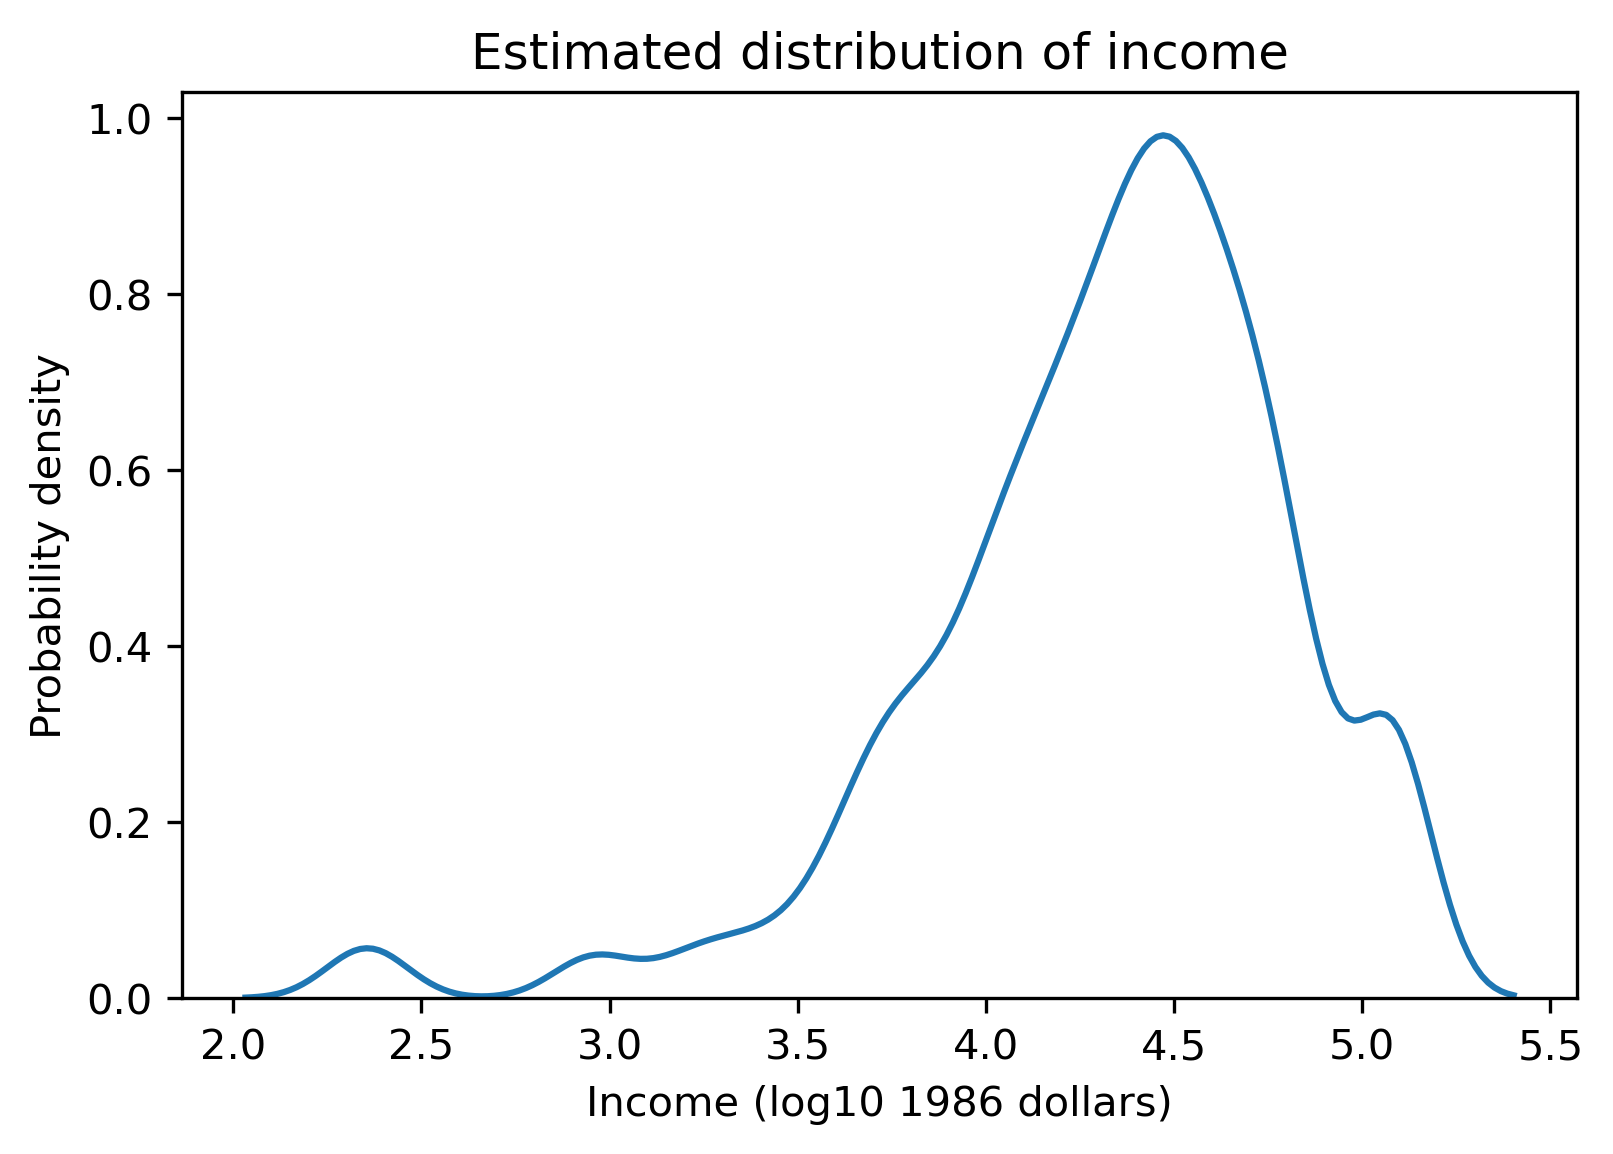
\includegraphics[width=4in]{12_bootstrap_files/12_bootstrap_115_0.png}
\end{center}

To draw samples from this distribution, we'll use a Scipy function
called \passthrough{\lstinline!gaussian\_kde!}, which takes the data and
returns an object that represents the estimated density.

\begin{lstlisting}[]
from scipy.stats import gaussian_kde

kde = gaussian_kde(log_realinc)
\end{lstlisting}

\passthrough{\lstinline!kde!} provides a method called
\passthrough{\lstinline!resample!} that draws random values from the
estimated density. As we've done in previous examples, we'll generate a
resampled dataset with the same size as the original.

\begin{lstlisting}[]
n = gss2018['REALINC'].notna().sum()
n
(@\dashfill@)
@@@2152@@@
\end{lstlisting}

Now we can draw a sample, compute the 10th percentile, and convert from
a logarithm to a dollar value.

\begin{lstlisting}[]
sample = kde.resample(n)
10 ** np.percentile(sample, 10)
(@\dashfill@)
@@@4961.50992778821@@@
\end{lstlisting}

The result is a random value from the sampling distribution of the 10th
percentile. The following function encapsulates these steps.

\begin{lstlisting}[]
def resample_kde_percentile(kde):
    sample = kde.resample(kde.n)
    return 10 ** np.percentile(sample, 10)
\end{lstlisting}

Now we can generate a sample from the sampling distribution.

\begin{lstlisting}[]
t10 = [resample_kde_percentile(kde)
       for i in range(1000)]

summary10 = summarize(t10)
\end{lstlisting}

The following table compares the results with KDE resampling to the
previous result with bootstrapping.

\begin{lstlisting}[]
table = pd.concat([summary9, summary10])
table.index=['bootstrapping', 'KDE resampling']
table
\end{lstlisting}

\begin{tabular}{lrrl}
\midrule
{} &  Estimate &      SE &               CI90 \\
\midrule
bootstrapping  &   5160.22 &  237.99 &   [5107.5, 5107.5] \\
KDE resampling &   5097.27 &  247.90 &  [4682.64, 5508.9] \\
\midrule
\end{tabular}

The means and standard errors are about the same with either method. The
difference is that the confidence interval we get from KDE resampling is
much more reasonable.

\hypertarget{summary}{%
\section{Summary}\label{summary}}

There are ten examples in this chapter so far; let's review them:

\begin{enumerate}
\def\labelenumi{\arabic{enumi}.}
\item
  First we used resampling based on a normal model to estimate average
  family income in the GSS and compute a confidence interval.
\item
  Then we used the same method to estimate the 10th percentile of
  income, and we found that the width of the confidence interval was 0.
  The problem is that the normal model does not fit the distribution of
  income.
\item
  To solve this problem, we switched to bootstrap sampling. First we
  estimated average family income and confirmed that the results are
  consistent with the results based on the normal model.
\item
  Then we used bootstrapping to estimate the 10th percentile of income.
  The results are much more plausible.
\item
  Next we used data from the BRFSS to estimate the average height of men
  in the U.S. Since this dataset is large, the confidence interval is
  very small. That means that the estimate is precise, in the sense that
  variability due to random sampling is small, but we don't know whether
  it is accurate, because there are other possible sources of error.
\item
  One of those sources of error is oversampling; that is, some people
  are more likely to appear in the sample than others. In the BFRSS,
  each respondent has a sampling weight that indicates how many people
  in the population they represent. We used these weighted to do
  weighted bootstrapping, and found that the error due to oversampling
  is larger than the variability due to random sampling.
\item
  In one exercise you used weighted bootstrapping to estimate the
  correlation of height and weight and compute a confidence interval.
\item
  In another exercise you estimated the slope of a regression line and
  computed a confidence interval.
\item
  Finally, I demonstrated a problem with bootstrap sampling when the
  dataset has only a few different values,
\item
  And presented a solution using KDE to smooth the data and draw samples
  from an estimated distribution.
\end{enumerate}

In the exercise below, you can work on one more example.

\textbf{Exercise:} In Chapter 10 we used logistic regression to model
support for legalizing marijuana as a function of age, sex, and
education level. Going back to that example, let's explore changes in
support over time and generate predictions for the next decade.

To prepare the data for logistic regression, we have to recode the
\passthrough{\lstinline!GRASS!} column so \passthrough{\lstinline!1!}
means in favor of legalization and \passthrough{\lstinline!0!} means not
in favor.

\begin{lstlisting}[]
gss['GRASS'].replace(2, 0, inplace=True)
gss['GRASS'].value_counts()
\end{lstlisting}

\begin{tabular}{lr}
\midrule
{} &  GRASS \\
\midrule
0.0 &  25662 \\
1.0 &  11884 \\
\midrule
\end{tabular}

As explanatory variables we'll use \passthrough{\lstinline!YEAR!} and
\passthrough{\lstinline!YEAR!} squared, which I'll store in a column
called \passthrough{\lstinline!YEAR2!}.

\begin{lstlisting}[]
gss['YEAR2'] = (gss['YEAR']-1990) ** 2
\end{lstlisting}

Now we can run the model like this:

\begin{lstlisting}[]
import statsmodels.formula.api as smf

formula = 'GRASS ~ YEAR + YEAR2'
results = smf.logit(formula, data=gss).fit(disp=False)
\end{lstlisting}

To generate predictions, I'll create a
\passthrough{\lstinline!DataFrame!} with a range of values of
\passthrough{\lstinline!YEAR!} up to 2030, and corresponding values of
\passthrough{\lstinline!YEAR2!}.

\begin{lstlisting}[]
years = np.linspace(1972, 2030)
df_pred = pd.DataFrame()
df_pred['YEAR'] = years
df_pred['YEAR2'] = (df_pred['YEAR']-1990)**2

pred = results.predict(df_pred)
\end{lstlisting}

I'll use \passthrough{\lstinline!groupby!} to compute the fraction of
respondents in favor of legalization during each year.

\begin{lstlisting}[]
grass_by_year = gss.groupby('YEAR')['GRASS'].mean()
\end{lstlisting}

The following function plots the data and decorates the axes.

\begin{lstlisting}[]
def plot_data():
    grass_by_year.plot(style='o', alpha=0.5, label='data')
    plt.xlabel('Year')
    plt.ylabel('Fraction in favor')
    plt.title('Support for legalization of marijuana')
    plt.legend(loc='upper left');
\end{lstlisting}

Here's what the predictions look like, plotted along with the data.

\begin{lstlisting}[]
plt.plot(years, pred, label='logistic model', color='gray')
plot_data()
\end{lstlisting}

\begin{center}
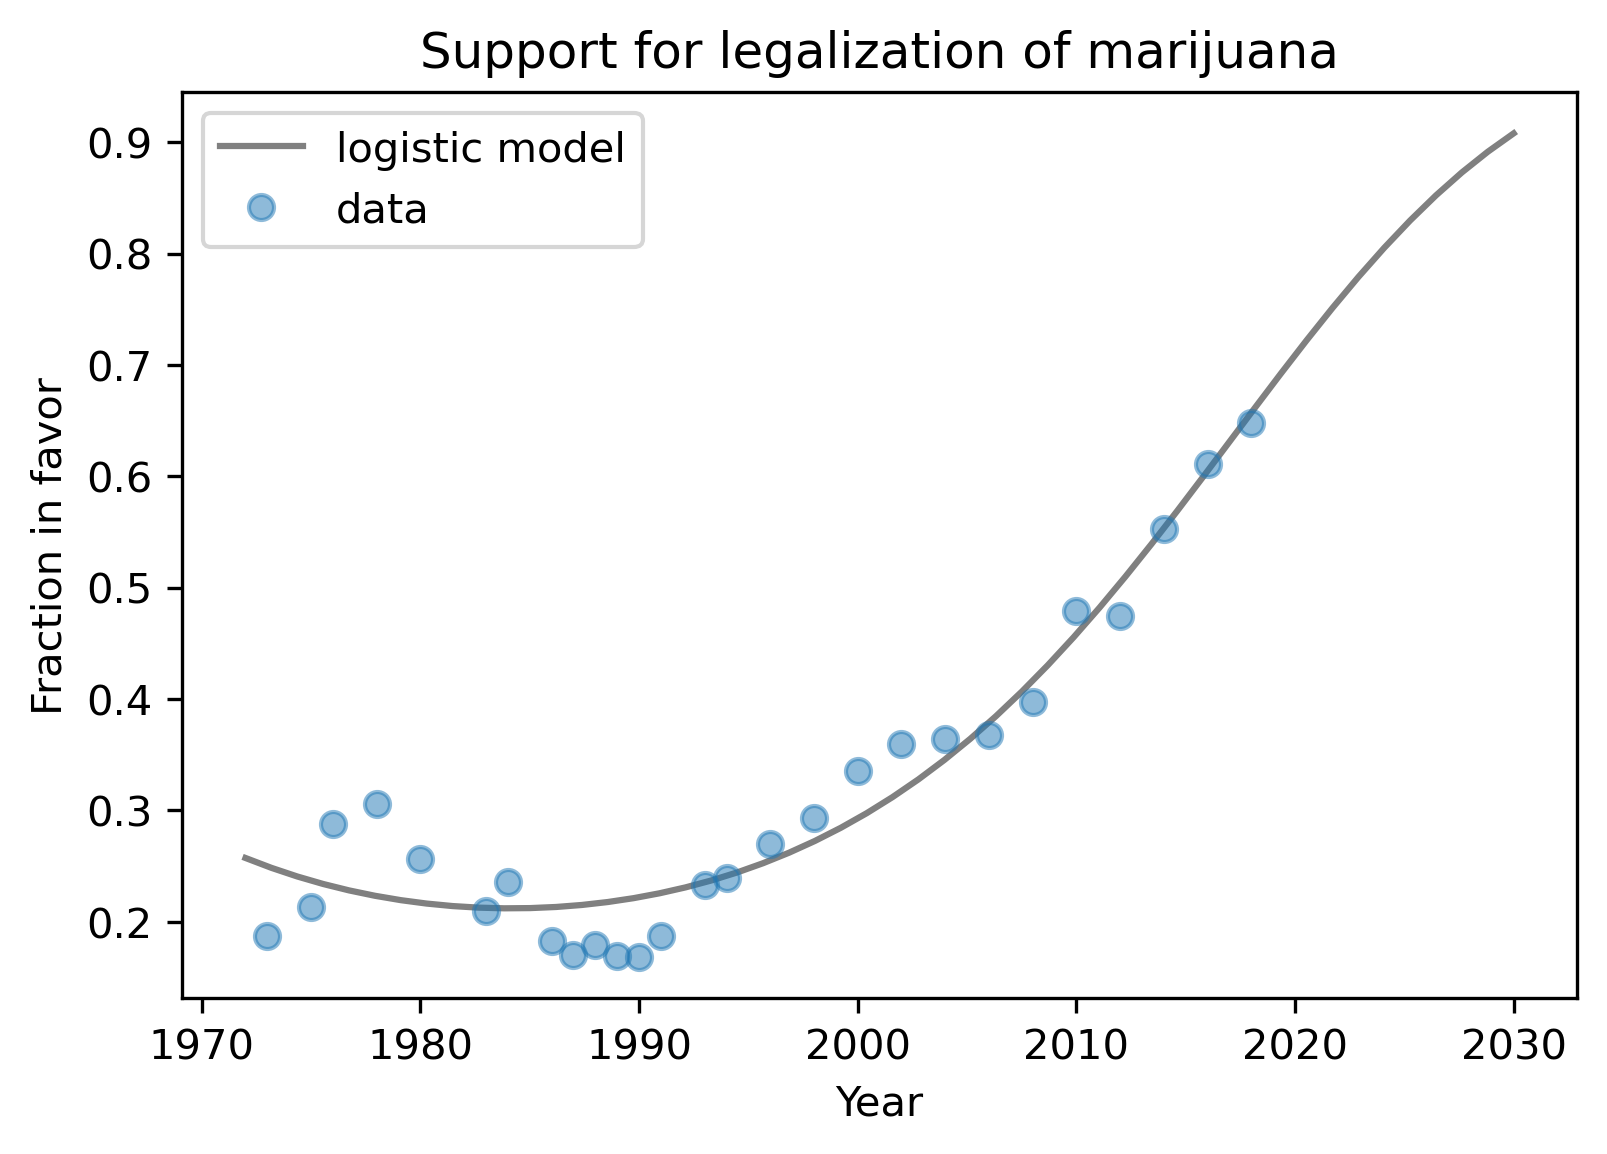
\includegraphics[width=4in]{12_bootstrap_files/12_bootstrap_144_0.png}
\end{center}

The model fits past data reasonably well and makes plausible predictions
for the next decade, although we can never be sure that trends like this
will continue.

This way of representing the results could be misleading because it does
not show our uncertainty about the predictions. Random sampling is just
one source of uncertainty among many, and for this kind of prediction it
is certainly not the biggest. But it is the easiest to quantify, so
let's do it, if only as an exercise.

Write a function called
\passthrough{\lstinline!bootstrap\_regression\_line!} that takes a
\passthrough{\lstinline!DataFrame!} as a parameter, uses
\passthrough{\lstinline!sample!} to resample the rows, runs the logistic
regression model, generates predictions for the rows in
\passthrough{\lstinline!df\_pred!}, and returns the predictions.

Call this function 101 times and save the results as a list of
\passthrough{\lstinline!Series!} objects. To visualize the results, you
have two options:

\begin{enumerate}
\def\labelenumi{\arabic{enumi}.}
\item
  Loop through the list and plot each prediction using a gray line with
  a low value of \passthrough{\lstinline!alpha!}. The overlapping lines
  will form a region showing the range of uncertainty over time.
\item
  Pass the list of \passthrough{\lstinline!Series!} to
  \passthrough{\lstinline!np.percentile!} with the argument
  \passthrough{\lstinline!axis=0!} to compute the 5th and 95th
  percentile in each column. Plot these percentiles as two lines, or use
  \passthrough{\lstinline!plt.fill\_between!} to plot a shaded region
  between them.
\end{enumerate}

